\documentclass{beamer}
\usepackage{lsfolien}
\usepackage[english]{babel}
\usepackage[utf8]{inputenc}

\myfootline{System Modelling and Semantic Web -- Spring 2021}{Hans-Gert Gräbe}

\newcommand{\ueberschrift}[1]{\begin{center}\bf #1\end{center}}

\title{Modelling Sustainable Systems\\ and Semantic Web\\[6pt]
  Digital Space of Action
  \vskip1em}

\subtitle{Lecture in the Module 10-202-2309\\ for Master Computer Science}

\author{Prof. Dr. Hans-Gert Gräbe\\
\url{http://www.informatik.uni-leipzig.de/~graebe}}

\date{May 2021}
\begin{document}

{\setbeamertemplate{footline}{}
\begin{frame}
  \titlepage
\end{frame}}

\section{World and Reality}
\begin{frame}{World and Reality}

  \begin{minipage}{.4\textwidth}\centering
    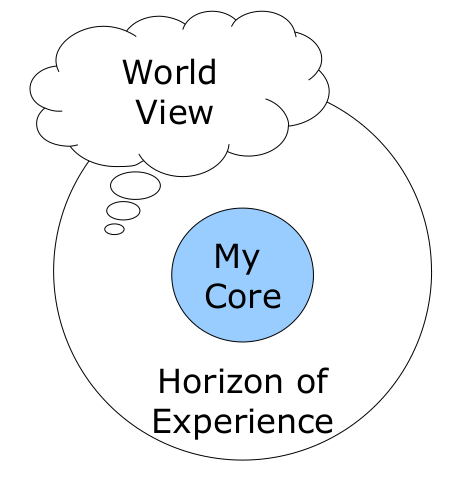
\includegraphics[width=\textwidth]{DI-1.png}
  \end{minipage}\hfill
  \begin{minipage}{.55\textwidth}
    \ueberschrift{Private and Cooperative Action}
    \begin{itemize}
    \item Art of living versus dealing with a structured world in a structured
      way
    \item Unpredictability versus predictability
    \item Constructability of "world“
    \item Me as a constructor
    \item (My) imagination and reality
    \end{itemize}
  \end{minipage}

\end{frame}
\begin{frame}{World and Reality}\centering
    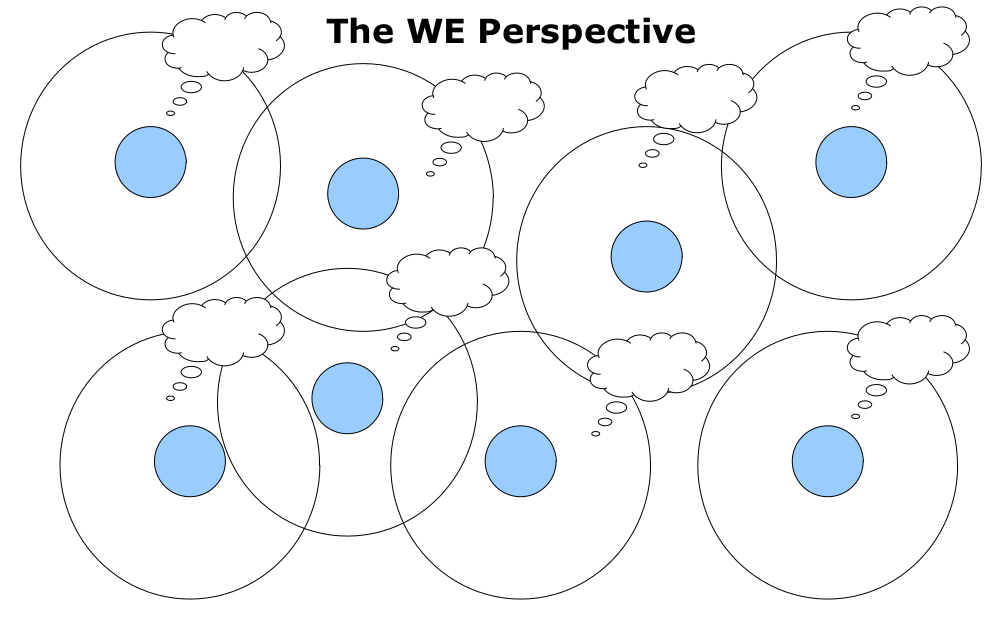
\includegraphics[width=.9\textwidth]{DI-2.png}
\end{frame}
\begin{frame}{World and Reality}\centering
    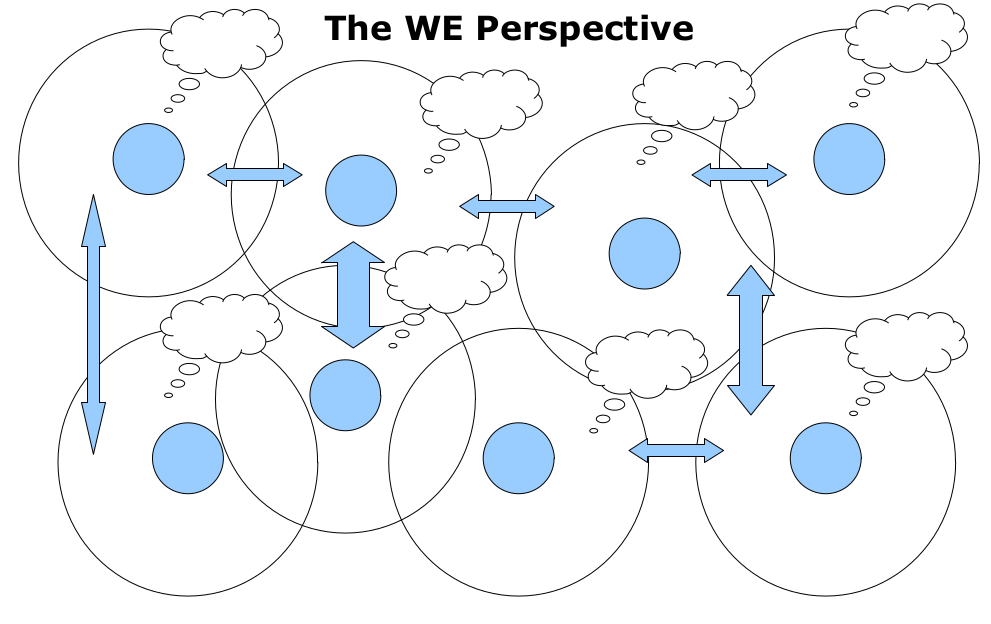
\includegraphics[width=.9\textwidth]{DI-3.png}
\end{frame}
\begin{frame}{World and Reality. Starting Point}
  \begin{itemize}
  \item Forms of description (plural) and reality.
  \item Contradictoriness of the world (as reality perceived by us)
  \item Differences in the concept of \emph{contradiction} in forms of
    description and forms of actions
  \item Descriptions and contextualisations
    \begin{itemize}
    \item Creativity and conceptualisation
    \item Concepts are a form of cooperative practices of people and thus
      themselves to be \emph{contextualised in a concrete-historical way}.
    \end{itemize}
  \item Term \emph{World View} for the complex context of the model-like
    reference \emph{in the model} to reality.
  \end{itemize}
  \begin{block}{World and Reality}
    \emph{World} is \emph{reality for us} and thus \emph{reality in the
      process of conceptual comprehension}.
  \end{block}
\end{frame}
\begin{frame}{World and Reality. What is Data?}
  \begin{itemize}
  \item Data as a specific form of description.
  \item Capturing data always means choosing what \emph{not} to capture.
  \item Data as a link between world and reality.
  \item But what then is \emph{objective} data?
    \begin{itemize}
    \item Specific reflex of a positivistic understanding of science.
    \item Use and misuse: Such an understanding (of science) is an important
      cultural achievement of humankind, which, however, also has to be
      \emph{contextualised in concrete-historical terms}.
    \end{itemize}
  \item Thus data is also a form of cooperative practices of people.
  \end{itemize}
\end{frame}

\section{The Digital Universe}
\begin{frame}{Digital Transformation}
  Concept of the \textbf{Digital Universe} as a rather technically shaped
  inner-societal space of action through the processing of digital data, with
  a vague demarcation.  Picking up a common buzz word.
\begin{itemize}
\item "By 2020, the digital universe will amount to 44 trillion gigabytes"
  (EMC Digital Universe with Research \& Analysis by IDC. The Digital Universe
  of Opportunities: Rich Data and the Increasing Value of the Internet of
  Things. April 2014).
\item Reference to the central thesis -- a spatial metaphor is used to analyse
  the digital transformation from a specific dichotomy.
\end{itemize}
\begin{block}{Central Thesis:}
  The digital transformation is characterised by a rapidly growing "world of
  digital data", through the analysis and processing of which influence is
  exerted on real-world processes.
\end{block}
\end{frame}
\begin{frame}{Digital Transformation}
  \ueberschrift{On the Critique of this Approach}
  \begin{itemize}
  \item In this version, we want to focus on questions of how current
    structuring processes in the digital universe and real-world processes
    interact and influence each other.
  \item The concept of juxtaposing "real-world" and "digital" reality is
    problematic overall, since actions in the digital universe are both
    motivated by real-world practices and have an influence on real-world
    practices.
 \item However, the concept emphasises that many real-world contexts of action
   interact with technical processes in this space and therefore such an
   abstraction seems reasonable.
  \end{itemize}
\end{frame}
\begin{frame}{Digital Transformation}
  \ueberschrift{The Digital Knowledge Revolution}

Michael Schetsche: "The digital knowledge revolution" (2006, in German)
identifies six social and cultural dimensions:
\begin{itemize}
\item a new order of knowledge,
\item social control through technical norms,
\item the automatic archive function of the net,
\item the supplementation of the exchange economy by a gift economy,
\item the abolition of the guiding difference between "public" and "private“, 
\item the dialectic of possibility and obligation of permanent communication.
\end{itemize}
\end{frame}
\begin{frame}{Digital Transformation}

All in all, it makes sense and is necessary to speak of a \emph{transformed
  social order} in which the \emph{structurally decisive changes} emanate from
the digital networks.

  A more precise understanding of the change in particular in the order of
  knowledge is an essential part of an analysis of the digital transformation.

  Problem: For the new phenomena, we (initially) only have the old terms.

  I will not elaborate on that here and refer to (Schetsche 2006).

\end{frame}

\section{Digital Spaces of Action}
\begin{frame}{Digital Spaces of Action}\centering\Large\bf

  How and where are you acting\\ in the digital universe?

  What opportunities for your own\\ and collective action in the digital
  universe\\ do you frequently use?

  Which preconditions\\ must be fulfilled for this?
\end{frame}
\begin{frame}{Digital Spaces of Action. From earlier Discussions}
  \begin{itemize}
  \item The digital universe breaks down into different universes -- the
    Instagram universe, the Facebook universe, the Google Scholar universe,
    the Wikipedia universe, the Search universe etc.
    \begin{itemize}
    \item Space in space metapher. Such „subspaces“ are constituted by specific
      kinds of social relations and specific social practices.
    \end{itemize}
  \item What to do there?
    \begin{itemize}
    \item Upload pictures and data.
    \item Like and be liked.
    \item Communcate with friends in Corona times.
    \item Online appointment for offline meeting.
    \item Present oneself in digital spaces.
    \item Searching for useful information.
    \end{itemize}
  \end{itemize}
\end{frame}
\begin{frame}{Digital Spaces of Action. Accounts}
  \begin{itemize}
  \item Diversity of accounts = diversity of digital identities
    \begin{itemize}
    \item Identity in the singular or in the plural?
    \item My Core -- world and reality, meaningful terms?
    \item Diversity of identities or of real-world facets
    \end{itemize}
  \item \emph{Identity} as an important concept in the civil legal system,
    which is also legally attached in order to be able to assign consequences
    of actions.
\item Questions of private digital spaces of action can only be meaningfully
  discussed if the user is "logged in" to a computer via an \textbf{account}.

  This also applies to other (e.g. mobile) devices, although the technical
  connection to an account (via SIM card and own security settings) is less
  visible there.
  \end{itemize}
\end{frame}
\begin{frame}{Using Digital Spaces of Action. Digital Identity}  
\begin{itemize}
\item Such an account is associated with a \textbf{digital identity} to which
  actions on the internet are assigned, via which the usual legal-social
  constructs of the \emph{legal attributability of actions} are transferred to
  the digital sphere.  
  \begin{itemize}
  \item The private attribution of consequences of action is a \emph{pillar of
    the civil legal order}.
  \item The technical possibilities in the digital universe can \emph{improve}
    or \emph{complicate} the attributability of legal responsibility.
  \item Possibility of \emph{anonymous action}. But: traces of actions are
    fundamentally accessible to forensic analysis. This also applies to
    actions on the internet.
  \end{itemize}
\end{itemize}
\end{frame}
\begin{frame}{Real-world and Digital Identities}
  \begin{center}
    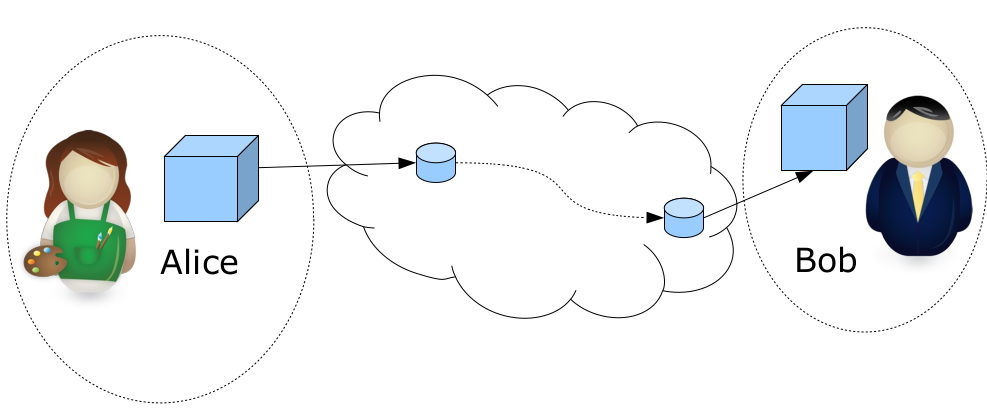
\includegraphics[width=.9\textwidth]{DI-4.png}
  \end{center}
  For actions in the digital universe, real-world identities must be tied to
  digital identities.
\end{frame}
\begin{frame}{Real-world and Digital Identities}
\begin{itemize}
\item The assignment of a digital identity to a real person takes place via
  \textbf{authentication}, which appears to be a \emph{private} act (albeit
  technically preconditioned).
  \begin{itemize}
  \item However, it presupposes an \textbf{authenticator} as the technical
    counterpart and thus a higher-level legal context. This assignment process
    is nevertheless postulated as private in the public.
  \end{itemize}
\item Private digital spaces of action can only be shaped through the
  binding to a digital identity.
  \begin{itemize}
  \item The rebinding of a digital identity to a civic legal subject is itself
    a socio-technically institutionalised process.
  \item This rebinding is particularly simple if the signature of a technical
    artefact from the digital universe can be easily assigned to the civil
    legal subject.
  \end{itemize}
\end{itemize}
\end{frame}
\begin{frame}{Acting on the Internet}\small
\begin{itemize}
\item Spaces of action are socially determined. Digital spaces of action can
  be and are constituted and assigned through \textbf{authorisation}.
\item In shaping spaces of action on the internet, subjects are highly
  dependent on technical services and thus on external institutions whose
  \emph{trustworthiness} they must assess appropriately.
\item Regulatory provisions for action on the internet exist only in
  rudimentary form, so that \emph{appropriate practical action} and
  \emph{cooperative arrangements} on a \emph{contractual basis} are the main
  forms of shaping a concept of "privacy on the internet".
\item An \emph{appropriate} understanding of the technical conditions,
  possibilities and restrictions of the internet is essential for the
  qualified shaping of personal actions on the internet.
\item Social action constitutes the intersubjective relations of a subject.
\end{itemize}
\end{frame}
\begin{frame}{On the Concept of Action Space}
  \begin{block}{Thesis:}
    The concept of action space in the nowadays common sense is a cultural
    achievement of bourgeois civic society.
  \end{block}\small
\begin{itemize}
\item Spaces of action as a "space within space" contextualise possibilities
  of cooperative arrangements in an "external space".
\item \emph{My} spaces of action are identity-constituting, and the actions in
  these spaces form the basis for my personality as a civic legal subject.
\item Only on this basis can delimitations of other concepts such as
  \emph{environment}, \emph{acting in an environment}, \emph{cooperative
    action} and thus ultimately concepts such as \emph{subject},
  \emph{privacy} and \emph{identity} be meaningfully grasped.
\item Collaborative spaces of action can be condensed into "cooperative
  subjects" in the sense of the civil legal order.
\end{itemize}
\end{frame}
\begin{frame}{Private Action and (Digital) Identity}

\emph{Private action} presupposes a \emph{concept of self}, of personal
\emph{identity}.
\begin{itemize}
\item Digital identity, multiple digital identity and roles
  \begin{itemize}
  \item[] Is identity divisible?
  \end{itemize}
\item Abstract identity, textual representation
  \begin{itemize}
  \item[] Assignment mechanisms, e.g. website and login
  \end{itemize}
\item Authentication
  \begin{itemize}
  \item[] Password, other forms of authentication
  \end{itemize}
\item Authorisation
  \begin{itemize}
  \item[] Me as subject and as object of authorisation.
  \end{itemize}
\item Potential and real assignment. Notion of session.
\end{itemize}
\end{frame}
\begin{frame}{Digital Identities}
\begin{itemize}
\item Digital identity, abstract identity, textual representation
\item Website, login, mobile devices
\item Concept of session (not only on websites)
\item Authentication and authorisation
\end{itemize}
\begin{block}{Digital Identity}
  In the following, we will understand \emph{digital identity} as a
  \textbf{real-world civic subject} \emph{authenticated} under a textual
  representation \texttt{<name@rechnername>} and \emph{authorised} in the
  context of a session, who performs actions in the digital universe for a
  limited period of time.
\end{block}
\end{frame}
\begin{frame}{Digital Identities and Roles}
  \ueberschrift{The Concept of Roles in Computer Science}
  
\begin{itemize}
\item In computer science, a role is a bundle of necessary \emph{experience,
  knowledge and skills} that an employee must have in order to perform a
  certain \emph{activity}.
\item Roles are defined by \emph{role descriptions} within a \emph{role
  model}.
\item A role is associated with \emph{activities} and \emph{responsibilities}.
\item \emph{Qualification characteristics} are required to perform a role.
\item A person can have several roles. Several persons can have the same role.
\end{itemize}
\end{frame}
\end{document}
